\section{Теоретические сведения}
\subsection{D-Bus}
D-Bus представляет из себя систему межпроцессорного взаимодействия, которая позволяет приложениям, находящимся в операционной системе (ОС), общаться между собой. D-Bus является частью проекта freedesktop.org~\cite{DBus}. Данная система обладает высокой скоростью работы, не зависит от рабочей среды и работает на POSIX-совместимых ОС.

D-Bus предоставляет несколько шин:
\begin{itemize}
\item Системная шина. Создается при старте демона D-Bus. С ее помощью происходит общение между различными демонами. 
\item Сессионная шина. Создается для пользователя, авторизовавшегося в системе. Для каждой сессионной шины запускается отдельная копия демона. Посредством этой копии общаются приложения, с которыми работает пользователь.
\end{itemize}

Каждое сообщение, передоваемое по шине, имеет своего отправителя. В том случае, когда сообщение не является широковещательным сигналом, оно имеет, в добавок к отправителю, своего получателя. Адреса отправителей и получаетлей, в контексте D-Bus, называются путями объектов по той причине, что каждое приложение состоит из набора объектов и сообщение происходит именно между этими объектами, а не между приложениями.

D-Bus также предусматривает концепцию сервисов. Сервис — уникальное местоположение приложения на шине. Приложение, при запуске, регистрирует один или несколько сервисов, которыми оно будет владеть до тех пор, пока самостоятельно не освободит. До этого момента никакое другое приложение, претендующее на тот же сервис, занять его не сможет. Именуются сервисы аналогично интерфейсам. После закрытия приложения ассоциированные сервисы также удаляются, а D-Bus посылает сигнал о том, что сервис закрыт.

Сервисы делают доступной ещё одну функцию — запуск необходимых приложений в случае поступления сообщений для них. Для этого должна быть включена автоактивация, а в конфигурации D-Bus за этим сервисом должно быть закреплено одно приложение.

После подключения к шине, приложение должно указать, какие сообщения оно желает получать, путём добавления масок совпадений (matchers). Маски представляют собой наборы правил для сообщений, которые будут доставляться приложению. Фильтрация может основываться на интерфейсах, путях объектов и методах.

Сообщения в D-Bus бывают четырёх видов: \textit{вызовы методов}, \textit{результаты вызовов методов}, \textit{сигналы (широковещательные сообщения)} и \textit{ошибки}.

В D-Bus у каждого объекта своё уникальное имя, которое выглядит как путь в файловой системе. Архитектура D-Bus показана с импользованием D-Bus интерфейса \textit{org.freedesktop.DBus.ObjectManager} на рис. \ref{fig:dbus}.
\begin{figure}[H]
\center{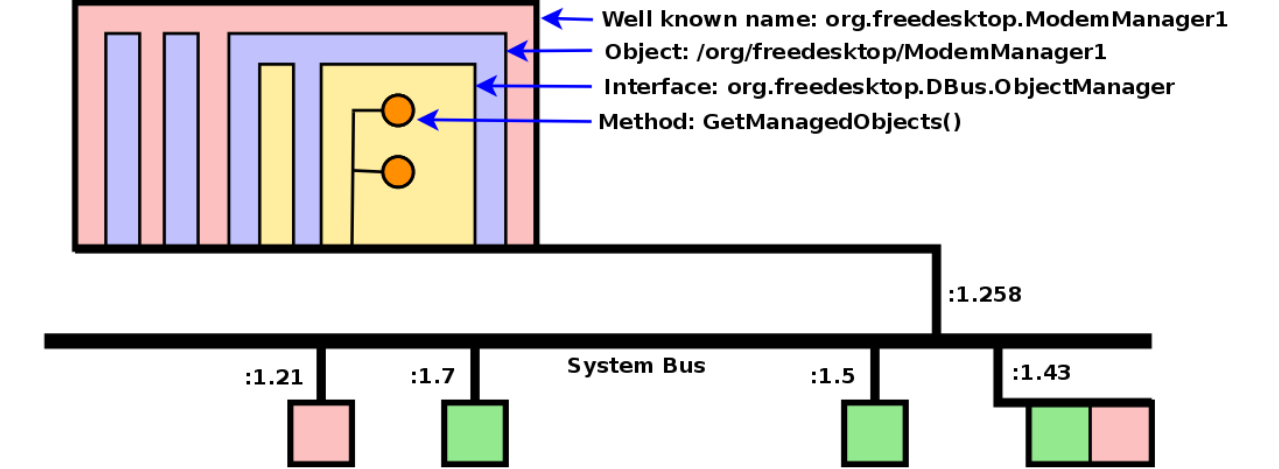
\includegraphics[width=0.6\linewidth]{dbus}}
\caption{Архитектура D-Bus}
\label{fig:dbus}
\end{figure}
\subsection{oFono}
Для организации общения с используемым sim-модулем был использолван программный проект oFono. Данный проект является бесплатным и распространяется под лицензией GNU GPL v2~\cite{oFono}. Проект oFono построен на стандарте 3GPP (3rg Generation Partnership Project) и использует D-Bus API для общения. Архитектура проекта oFono показана на рис. \ref{fig:ofono}.
\begin{figure}[H]
\center{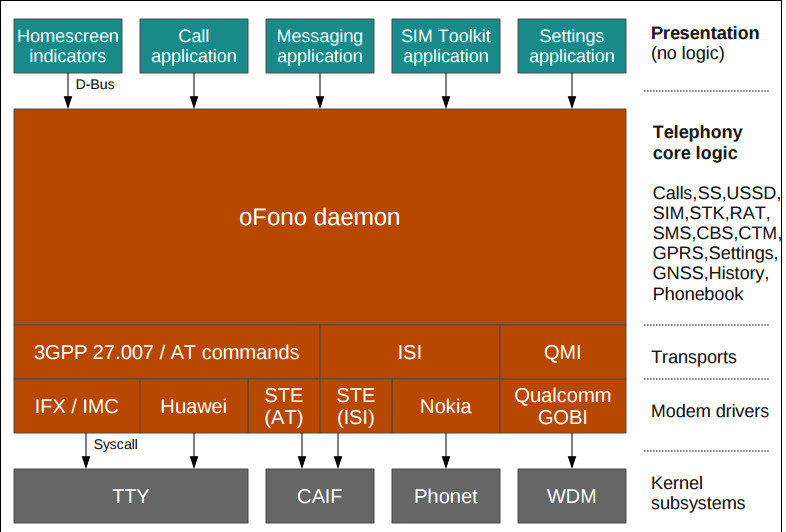
\includegraphics[width=0.6\linewidth]{ofono}}
\caption{Архитектура ofono}
\label{fig:ofono}
\end{figure}

Проект oFono был анонсирован компаниями Intel и Nokia в мая 2009 года. Последняя версия 1.4 была представлена в августе 2016 года. Работа над данным проектом ведется до сих пор. Исходные коды oFono находятся в свободном доступе, в гит репозитории~\cite{oFonoSources}.

Программный стек oFono поддерживает различные модули, такие как:
\begin{itemize}
\item 2G/3G
\item LTE
\item CDMA(Code-division multiple access)
\item GSM
\item Bluetooth и т.д.
\end{itemize}

Общаение между oFono и sim-модулем будет производится через различные AT-команды. В свою очередь, разрабатываемый демон будет общаться с oFono посредством D-Bus.
